%!TEX program = xelatex

\documentclass[a4paper, openany, oneside]{memoir}
\usepackage[no-math]{fontspec}
\usepackage{pgfplots}
\pgfplotsset{compat=newest}
\usepackage{commath}
\usepackage{mathtools}
\usepackage{amssymb}
\usepackage{amsthm}
\usepackage{booktabs}
\usepackage{mathtools}
\usepackage{xcolor}
\usepackage[separate-uncertainty=true, per-mode=symbol]{siunitx}
\usepackage[noabbrev, capitalize]{cleveref}
\usepackage{listings}
\usepackage[american inductor, european resistor]{circuitikz}
\usepackage{amsmath}
\usepackage{amsfonts}
\usepackage{ifxetex}
\usepackage[dutch,english]{babel}
\usepackage[backend=bibtexu,texencoding=utf8,bibencoding=utf8,style=ieee,sortlocale=en_GB,language=auto]{biblatex}
\usepackage[strict,autostyle]{csquotes}
\usepackage{parskip}
\usepackage{import}
\usepackage{standalone}
\usepackage{hyperref}
%\usepackage[toc,title,titletoc]{appendix}

\ifxetex{} % Fonts laden in het geval dat je met Xetex compiled
    \usepackage{fontspec}
    \defaultfontfeatures{Ligatures=TeX} % To support LaTeX quoting style
    \setromanfont{Palatino Linotype} % Tover ergens in Font mapje in root.
    \setmonofont{Source Code Pro}
\else % Terug val in standaard pdflatex tool chain. Geen ondersteuning voor OTT fonts
    \usepackage[T1]{fontenc}
    \usepackage[utf8]{inputenc}
\fi
\newcommand{\references}[1]{\begin{flushright}{#1}\end{flushright}}
\renewcommand{\vec}[1]{\boldsymbol{\mathbf{#1}}}
\newcommand{\uvec}[1]{\boldsymbol{\hat{\vec{#1}}}}
\newcommand{\mat}[1]{\boldsymbol{\mathbf{#1}}}
\newcommand{\fasor}[1]{\boldsymbol{\tilde{\vec{#1}}}}
\newcommand{\cmplx}[0]{\mathrm{j}}
\renewcommand{\Re}[0]{\operatorname{Re}}
\newcommand{\Cov}{\operatorname{Cov}}
\newcommand{\Var}{\operatorname{Var}}
\newcommand{\proj}{\operatorname{proj}}
\newcommand{\Perp}{\operatorname{perp}}
\newcommand{\col}{\operatorname{col}}
\newcommand{\rect}{\operatorname{rect}}
\newcommand{\sinc}{\operatorname{sinc}}
\newcommand{\IT}{\operatorname{IT}}
\newcommand{\F}{\mathcal{F}}

\newtheorem{definition}{Definition}
\newtheorem{theorem}{Theorem}


\DeclareSIUnit{\voltampere}{VA} %apparent power
\DeclareSIUnit{\pii}{\ensuremath{\pi}}

\hypersetup{%setup hyperlinks
    colorlinks,
    citecolor=black,
    filecolor=black,
    linkcolor=black,
    urlcolor=black
}

% Example boxes
\usepackage{fancybox}
\usepackage{framed}
\usepackage{adjustbox}
\newenvironment{simpages}%
{\AtBeginEnvironment{itemize}{\parskip=0pt\parsep=0pt\partopsep=0pt}
\def\FrameCommand{\fboxsep=.5\FrameSep\shadowbox}\MakeFramed{\FrameRestore}}%
{\endMakeFramed}

% Impulse train
\DeclareFontFamily{U}{wncy}{}
\DeclareFontShape{U}{wncy}{m}{n}{<->wncyr10}{}
\DeclareSymbolFont{mcy}{U}{wncy}{m}{n}
\DeclareMathSymbol{\Sha}{\mathord}{mcy}{"58}
\addbibresource{../../../../includes/bibliography.bib}

\begin{document}

\section{Appendix: circular sparse ruler problem}
\label{ap:circ-ruler}
% We introduce the concept of a ruler. Consider a ruler $\vec{r}$ of length $N$, then vector $\mathbf{S}$ represents the locations on the ruler that are occupied by samplers. A circular sparse ruler contains a distance $d$ if there exist an $S_i$ and $S_j$ such that $|S_i-S_j| = d$ or  $N-|S_i-S_j| = d$. A solution to a circular ruler is correct if it contains lags $ 1, \ldots, N - 1$. \Cref{fig:circular-ruler} shows a circular sparse ruler for $N=7$. The circle depicts the ruler and contains $N$ ticks. Then $(\vec{r})_i = 1$ if the tick at position $i$ is red. The definition of a circular ruler then states that the ruler is circular if and only if the distances between the marks are the distances $1,\ldots,N-1$.

% In circular sparse ruler we have different samplers with the same sampling frequency $N$. Therefore the sampling structure is periodic with  period $N$.
% If we can make lag $L$ we can also make lag $L+kN$ with $k$ an integer. Therefore if we can make lags $\{0,1,\dots,N-1\}$, we can make all lags. This problem is called circular sparse ruler. 
The circular sparse ruler problem was introduced in \cref{cha:reconstruction} and reformulated in \cref{cha:sampling_methods}. Consider a circle with $N$ marks on it. Every mark is occupied by a sampler. Time on this circle passes as the hand of a clock. By continuity of the circle, the lag $d$ is estimated if the two marks are $d$ apart. The circle is illustrated in \cref{fig:circular-ruler}. Here $N=7$ and the positions $1$, $2$ and $3$ are marked. The circle is a solution to the circular sparse ruler problem, since the distances between the marks make up $0,\ldots,N-1$.

\begin{figure}
    \centering
    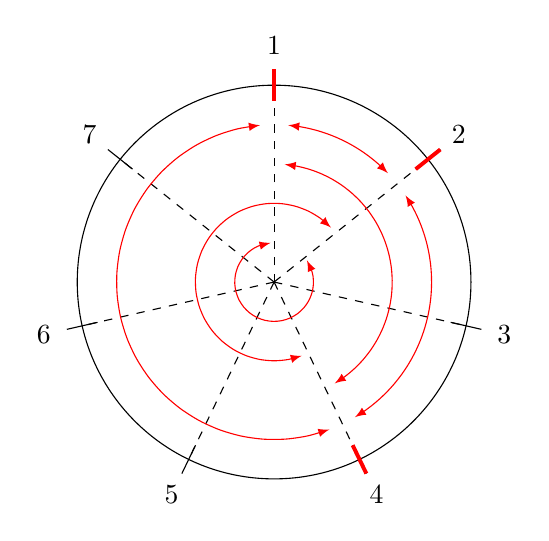
\begin{tikzpicture}
        \def\N{7}
        \draw [black] circle[radius=2.5cm] (0,0);
        \foreach \i in {1,...,\N} {
            \draw [scale=1,domain=2.3:2.7,smooth,variable=\x,black] plot ({\x*sin(360*(\i-1)/\N)},{\x*cos(360*(\i-1)/\N)});
            \draw [black,dashed] (0,0) -- ({2.5*sin(360*(\i-1)/\N)},{2.5*cos(360*(\i-1)/\N)});
            \node[black] at ({3*sin(360*(\i-1)/\N)},{3*cos(360*(\i-1)/\N)}) {$\i$};
        }
        \foreach \i in {0,1,3} {
            \draw [scale=1,domain=2.3:2.7,smooth,variable=\x,red,line width=0.5mm] plot ({\x*sin(360*\i/\N)},{\x*cos(360*\i/\N)});
        }
        \draw [scale=1,domain=0.1:0.9,smooth,variable=\x,black,>=latex,<->,red] plot ({2*sin(360*\x/\N)},{2*cos(360*\x/\N)}); % 1
        \draw [scale=1,domain=1.1:2.9,smooth,variable=\x,black,>=latex,<->,red] plot ({2*sin(360*\x/\N)},{2*cos(360*\x/\N)}); % 2
        \draw [scale=1,domain=3.1:6.9,smooth,variable=\x,black,>=latex,<->,red] plot ({2*sin(360*\x/\N)},{2*cos(360*\x/\N)}); % 4
        \draw [scale=1,domain=0.1:2.9,smooth,variable=\x,black,>=latex,<->,red] plot ({1.5*sin(360*\x/\N)},{1.5*cos(360*\x/\N)}); % 3
        \draw [scale=1,domain=3.1:7.9,smooth,variable=\x,black,>=latex,<->,red] plot ({1*sin(360*\x/\N)},{1*cos(360*\x/\N)}); % 5
        \draw [scale=1,domain=1.1:6.9,smooth,variable=\x,black,>=latex,<->,red] plot ({0.5*sin(360*\x/\N)},{0.5*cos(360*\x/\N)}); % 6
    \end{tikzpicture}
    \caption{Circular sparse ruler problem for $N=7$}
    \label{fig:circular-ruler}
\end{figure}

Finding solutions to the circular sparse ruler problem where the amount of marks is minimised is relevant to us, since a minimal amount of marks is equivalent to using a minimal amount of samplers for a given $N$. We call these solutions minimal circular sparse ruler solutions.

\cite{ariananda2012compressive} proposes a method that uses the so called linear sparse ruler problem to generate solution for the circular sparse ruler problem. The linear sparse ruler problem is similar to the circular sparse ruler problem. If one disconnects the end of the circle in \cref{fig:circular-ruler}, but still requires that the marks make up the distances $0,\ldots,N-1$, one obtains the linear sparse ruler problem. This is illustrated in \cref{tkz:linear_sparse_ruler}.  

\begin{figure}[H]
\centering
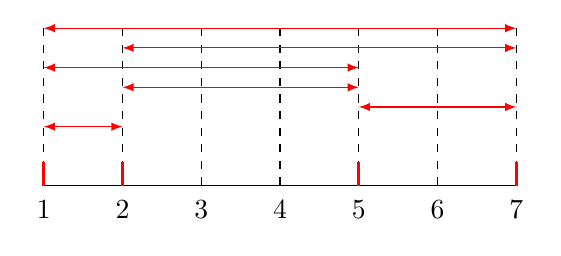
\begin{tikzpicture}

\draw (0,1) -- (6,1);

\foreach \i in {0,...,6} {
    \draw [dashed] (\i,1) -- (\i,3);
}


\draw [red, very thick] (0,1) -- (0,1.3);
\draw [red, very thick](1,1) -- (1,1.3);
% \draw (2,1) -- (2,1.1);
% \draw (3,1) -- (3,1.1);
\draw [red, very thick](4,1) -- (4,1.3);
% \draw (5,1) -- (5,1.1);
\draw [red, very thick](6,1) -- (6,1.3);


\draw [red, >=latex,<->] (0,1.75) -- (1,1.75);
\draw [red, >=latex,<->](4,2) -- (6,2);
\draw [red, >=latex,<->](1,2.25) -- (4,2.25);
\draw [red, >=latex,<->](0,2.5) -- (4,2.5);
\draw [red, >=latex,<->](1,2.75) -- (6,2.75);
\draw [red, >=latex,<->](0,3) -- (6,3);

\node at (0,0.7) {1};
\node at (1,0.7) {2};
\node at (2,0.7) {3};
\node at (3,0.7) {4};
\node at (4,0.7) {5};
\node at (5,0.7) {6};
\node at (6,0.7) {7};

\end{tikzpicture}
\caption{Linear sparse ruler for $N=7$ and $M=4$}\label{tkz:linear_sparse_ruler}
\end{figure}

The proposed method in \cite{ariananda2012compressive} uses the fact that a linear sparse solution for a certain $N$ can be turned into circular sparse ruler solutions for $2N-2$ when $N$ is even and $2N-1$ when $N$ is odd. To see this, simply note that every distance $d$ between marks on a circle also yields a distance $N-d$. The linear sparse solution in \cref{tkz:linear_sparse_ruler} is therefore also a circular sparse ruler solution for $N=13$. This is illustrated in \cref{tkz:circ_linear_sparse}. 

\begin{figure}[H]
\centering
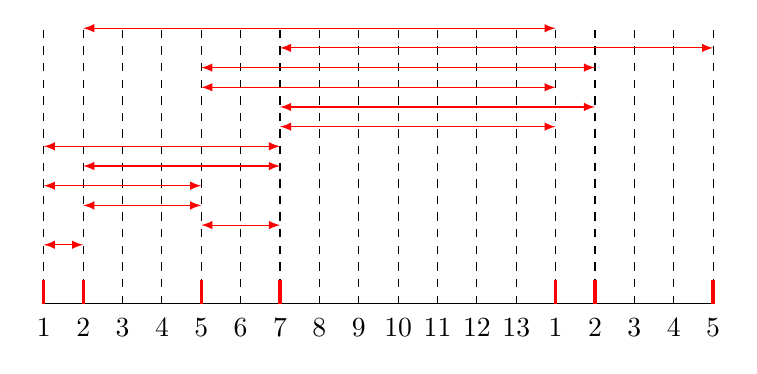
\begin{tikzpicture}

\foreach \i in {0,...,17} {
    \draw [dashed] (\i/2,1) -- (\i/2,4.5);
}



\draw (0,1) -- (8.5,1);

\draw [red, very thick] (0,1) -- (0,1.3);
\draw [red, very thick](.5,1) -- (.5,1.3);
% \draw (1,1) -- (1,1.1);
% \draw (1.5,1) -- (1.5,1.1);
\draw [red, very thick](2,1) -- (2,1.3);
% \draw (2.5,1) -- (2.5,1.1);
\draw [red, very thick](3,1) -- (3,1.3);
% \draw  (3.5,1) -- (3.5,1.1);
% \draw (4,1) -- (4,1.1);
% \draw (4.5,1) -- (4.5,1.1);
% \draw (5,1) -- (5,1.1);
% \draw (5.5,1) -- (5.5,1.1);
% \draw (6,1) -- (6,1.1);

\draw [red, very thick] (6.5,1) -- (6.5,1.3);
\draw [red, very thick](7,1) -- (7,1.3);
% \draw (7.5,1) -- (7.5,1.1);
% \draw (8,1) -- (8,1.1);
\draw [red, very thick](8.5,1) -- (8.5,1.3);

\draw [red, >=latex,<->] (0,1.75) -- (.5,1.75);
\draw [red, >=latex,<->](2,2) -- (3,2);
\draw [red, >=latex,<->](.5,2.25) -- (2,2.25);
\draw [red, >=latex,<->](0,2.5) -- (2,2.5);
\draw [red, >=latex,<->](.5,2.75) -- (3,2.75);
\draw [red, >=latex,<->](0,3) -- (3,3);
\draw [red, >=latex,<->](3,3.25) -- (6.5,3.25);
\draw [red, >=latex,<->](3,3.5) -- (7,3.5);
\draw [red, >=latex,<->](2,3.75) -- (6.5,3.75);
\draw [red, >=latex,<->](2,4) -- (7,4);
\draw [red, >=latex,<->](3,4.25) -- (8.5,4.25);
\draw [red, >=latex,<->](.5,4.5) -- (6.5,4.5);

\node at (0,0.7) {1};
\node at (.5,0.7) {2};
\node at (1,0.7) {3};
\node at (1.5,0.7) {4};
\node at (2,0.7) {5};
\node at (2.5,0.7) {6};
\node at (3,0.7) {7};
\node at (3.5,0.7) {8};
\node at (4,0.7) {9};
\node at (4.5,0.7) {10};
\node at (5,0.7) {11};
\node at (5.5,0.7) {12};
\node at (6,0.7) {13};
\node at (6.5,0.7) {1};
\node at (7,0.7) {2};
\node at (7.5,0.7) {3};
\node at (8,0.7) {4};
\node at (8.5,0.7) {5};

\end{tikzpicture}
\caption{Circular sparse solution for $N=13$ generated from the linear sparse ruler solution for $N=7$. The numbers on the axis repeat since this is a circular sparse ruler problem.}\label{tkz:circ_linear_sparse}
\end{figure}

The generation approach is advantageous, since solutions of linear sparse ruler problem can be turned into circular sparse ruler solutions. Therefore better linear sparse ruler solutions will also result in better circular sparse ruler solutions. Because linear sparse ruler is a well-known problem, good solutions are already calculated. However, solutions genererated for the circular sparse ruler problem are not necessarily minimal. Finding minimal solutions is by no means trivial and requires clever algorithms. It is also interesting to look at the structure of the problem to decrease the solution space.

\subsection{Structure of the circular sparse ruler problem}
Optimal circular sparse rulers form interesting solutions to the circular sparse ruler problem. They are circular sparse ruler solutions to configurations with $M$ samplers such that $N$ is as high as possible. Optimal solutions ensure the highest performance possible for a given amount of samplers. In similar fashion, one can define optimal solutions to the linear sparse ruler problem. 

\begin{blockTheorem}[Upper bound on circular sparse ruler solutions]\label{th:upperbound}
Consider a configuration with $M$ samplers. Then $N \le M(M-1)+1$.
\end{blockTheorem}

\begin{blockProofTheorem}{\ref{th:upperbound}}
    There are $M^2$ combinations of samplers. However, $M$ of them result in a combination with themself, which yields an estimation of lag $0$. Therefore, only $M^2-M+1=M(M-1)+1$ different lags can be estimated. The estimated lags must make up $0,\ldots,N-1$, which are $N$ different lags. Therefore $N \le M(M-1)+1$.
\end{blockProofTheorem}

\subsection{Results}
We have used integer linear programming to calculate circular sparse ruler solutions. This program is explained and derived in \cref{ap:derivation_ILP}. The solutions are shown in \cref{tab:circ-sols}.
\begin{table}
    \centering
    \begin{tabular}{lll}
        $M$ & $N$ & \textbf{Marks at positions} \\ \hline
        $2$ & $3$ & $1,2$ \\
        $3$ & $7$ & $1,2,4$ \\
        $4$ & $13$ & $1,2,5,7$ \\
        $5$ & $21$ & $1,2,7,9, 19$ \\
        $6$ & $31$ & $1,2,5,7,14,22$ \\
        $7$ & $39$ & $1,2,5,7,14,21,31$ \\
        $8$ & $51$ & $1,2,8,10,13,32,36, 46$ \\
        $9$ & $65$ & $1,2,5,7,15, 33, 43, 51, 54$ \\
    \end{tabular}
    \caption{Several solutions to the circular sparse ruler proble}
    \label{tab:circ-sols}
\end{table}

\Cref{fig:comparison_sparse_ruler} compares the upper bound from \cref{th:upperbound} to minimal linear sparse ruler solutions and minimal circular sparse ruler solutions. One can clearly see that for high $M$, minimal solutions to the circular sparse ruler problem have higher $N$.
% \begin{figure}[H]
% \begin{tikzpicture}
% \begin{axis}[xlabel={Number of samples ($M$)},ylabel={Downsampling factor ($N$)},width=\textwidth, height=0.8\textwidth]
%     \addplot [
%     color=green,
%     solid,
%     mark=.,
%     ]
%     %table[x index=0,y index=1,col sep=comma] {circ_upper.data};
%     table [col sep=comma]{plots/circ_upper.txt};
    
%     \addplot [
%     color=blue,
%     solid,
%     mark=.,
%     ]
%     % table[x index=0,y index=1,col sep=comma] {circ_ilp.data};
%     table [col sep=comma]{plots/circ_ilp.txt};

%     \addplot [
%     color=red,
%     solid,
%     mark=.,
%     ]
%     % table[x index=0,y index=1,col sep=comma] {circ_lin.data};
%     table [col sep=comma]{plots/circ_lin.txt};
% \end{axis}
% \end{tikzpicture}
% \caption{Solutions of the circular and linear sparse ruler problem. Minimal solutions to linear sparse ruler are shown in red, minimal solutions to the circular sparse ruler problem are shown in blue and the upper bound from \cref{th:upperbound} is shown in green.}\label{fig:comparison_sparse_ruler}
% \end{figure}

\section{Collaborative sampling}
Collaborative sampling also requires that the circular sparse ruler problem is satisfied. In this case, however, the estimation of the lags is split across two physically separate devices. This is shown in \cref{tkz:collaborative_ruler}.
\begin{figure}
\centering
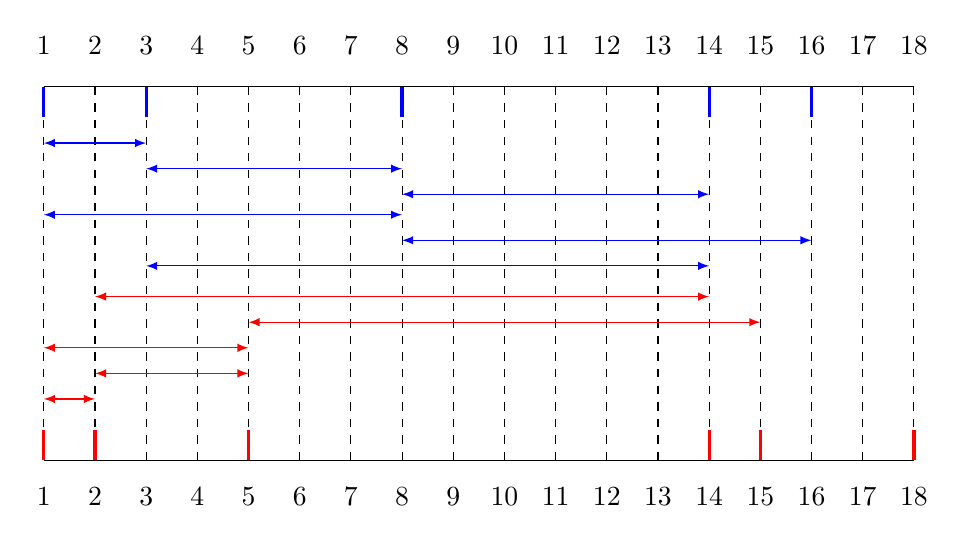
\begin{tikzpicture}[scale=1.3]
\foreach \i in {0,...,17} {
    \draw [dashed] (\i/2,-0.35) -- (\i/2,3.3);
}

\draw (0,3.3) -- (8.5,3.3);
\draw [blue, very thick] (0,3) -- (0,3.3);
% \draw (0.5,3.2) -- (0.5,3.3);
\draw [blue, very thick](1,3) -- (1,3.3);
% \draw (1.5,3.2) -- (1.5,3.3);
% \draw (2,3.2) -- (2,3.3);
% \draw (2.5,3.2) -- (2.5,3.3);
% \draw (3,3.2) -- (3,3.3);
\draw [blue, very thick](3.5,3) -- (3.5,3.3);
% \draw (4,3.2) -- (4,3.3);
% \draw (4.5,3.2) -- (4.5,3.3);
% \draw (5,3.2) -- (5,3.3);
% \draw (5.5,3.2) -- (5.5,3.3);
% \draw (6,3.2) -- (6,3.3);
\draw [blue, very thick] (6.5,3) -- (6.5,3.3);
% \draw (7,3.2) -- (7,3.3);
\draw [blue, very thick](7.5,3) -- (7.5,3.3);
% \draw (8,3.2) -- (8,3.3);
% \draw (8.5,3.2) -- (8.5,3.3);

\node at (0,3.7) {1};
\node at (0.5,3.7) {2};
\node at (1,3.7) {3};
\node at (1.5,3.7) {4};
\node at (2,3.7) {5};
\node at (2.5,3.7) {6};
\node at (3,3.7) {7};
\node at (3.5,3.7) {8};
\node at (4,3.7) {9};
\node at (4.5,3.7) {10};
\node at (5,3.7) {11};
\node at (5.5,3.7) {12};
\node at (6,3.7) {13};
\node at (6.5,3.7) {14};
\node at (7,3.7) {15};
\node at (7.5,3.7) {16};
\node at (8,3.7) {17};
\node at (8.5,3.7) {18};

\draw (0,-0.35) -- (8.5,-0.35);
\draw [red, very thick] (0,-0.35) -- (0,-0.05);
\draw [red, very thick](0.5,-0.35) -- (0.5,-0.05);
% \draw (1,-0.35) -- (1,-0.25);
% \draw (1.5,-0.35) -- (1.5,-0.25);
\draw [red, very thick](2,-0.35) -- (2,-0.05);
% \draw (2.5,-0.35) -- (2.5,-0.25);
% \draw (3,-0.35) -- (3,-0.25);
% \draw  (3.5,-0.35) -- (3.5,-0.25);
% \draw (4,-0.35) -- (4,-0.25);
% \draw (4.5,-0.35) -- (4.5,-0.25);
% \draw (5,-0.35) -- (5,-0.25);
% \draw (5.5,-0.35) -- (5.5,-0.25);
% \draw (6,-0.35) -- (6,-0.25);
\draw [red, very thick] (6.5,-0.35) -- (6.5,-0.05);
\draw [red, very thick](7,-0.35) -- (7,-0.05);
% \draw (7.5,-0.35) -- (7.5,-0.25);
% \draw (8,-0.35) -- (8,-0.25);
\draw [red, very thick](8.5,-0.35) -- (8.5,-0.05);

\node at (0,-0.7) {1};
\node at (0.5,-0.7) {2};
\node at (1,-0.7) {3};
\node at (1.5,-0.7) {4};
\node at (2,-0.7) {5};
\node at (2.5,-0.7) {6};
\node at (3,-0.7) {7};
\node at (3.5,-0.7) {8};
\node at (4,-0.7) {9};
\node at (4.5,-0.7) {10};
\node at (5,-0.7) {11};
\node at (5.5,-0.7) {12};
\node at (6,-0.7) {13};
\node at (6.5,-0.7) {14};
\node at (7,-0.7) {15};
\node at (7.5,-0.7) {16};
\node at (8,-0.7) {17};
\node at (8.5,-0.7) {18};

\draw [red, >=latex,<->] (0,0.25) -- (0.5,0.25);
\draw [blue, >=latex,<->](0,2.75) -- (1,2.75);
\draw [red, >=latex,<->](0.5,0.5) -- (2,0.5);
\draw [red, >=latex,<->](0,0.75) -- (2,0.75);
\draw [blue, >=latex,<->](1,2.5) -- (3.5,2.5);
\draw [blue, >=latex,<->](3.5,2.25) -- (6.5,2.25);
\draw [blue, >=latex,<->](0,2.05) -- (3.5,2.05);
\draw [blue, >=latex,<->](3.5,1.8) -- (7.5,1.8);
\draw [red, >=latex,<->](2,1) -- (7,1);
\draw [blue, >=latex,<->](1,1.55) -- (6.5,1.55);
\draw [red, >=latex,<->](0.5,1.25) -- (6.5,1.25);

\end{tikzpicture}
\caption{Collaborative sampling with $N=13$ and $M=4$}\label{tkz:collaborative_ruler}
\end{figure}
The red arrows indicate the lags that are produced by device one, and the blue arrows indicate the lags that are produced by device two. Note that together they make all lags available. \cite{ariananda2014cooperative} investigates ways to come up with optimal set-ups for different amounts of devices.

\section{Coprime sampling}
Similarly, coprime sampling also requires that the circular sparse ruler problem is satisfied. A configuration for coprime sampling is depicted in \cref{tkz:coprime_ruler}.

\begin{figure}
\centering
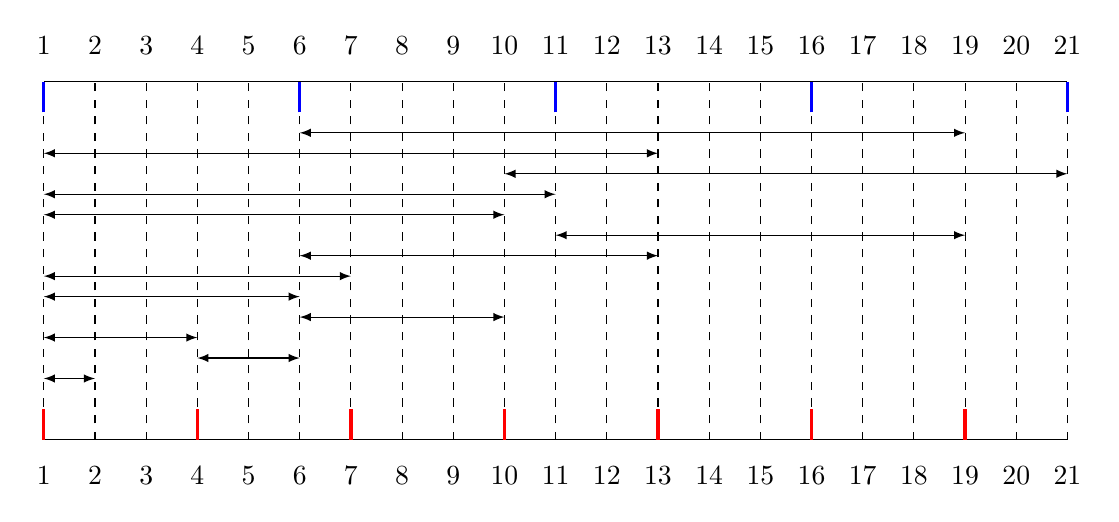
\begin{tikzpicture}[scale=1.3]

\foreach \i in {0,...,20} {
    \draw [dashed] (1+\i/2,0) -- (1+\i/2,3.5);
}

\draw (1,0) -- (11,0);

\draw [red, very thick] (1,0) -- (1,0.3);
% \draw (1.5,0) -- (1.5,0.1);
% \draw (2,0) -- (2,0.1);
\draw [red, very thick] (2.5,0) -- (2.5,0.3);
% \draw (3,0) -- (3,0.1);
% \draw (3.5,0) -- (3.5,0.1);
\draw [red, very thick] (4,0) -- (4,0.3);
% \draw  (4.5,0) -- (4.5,0.1);
% \draw (5,0) -- (5,0.1);
\draw [red, very thick] (5.5,0) -- (5.5,0.3);
% \draw (6,0) -- (6,0.1);
% \draw (6.5,0) -- (6.5,0.1);
\draw [red, very thick] (7,0) -- (7,0.3);
% \draw (7.5,0) -- (7.5,0.1);
% \draw (8,0) -- (8,0.1);
\draw [red, very thick] (8.5,0) -- (8.5,0.3);
% \draw (9,0) -- (9,0.1);
% \draw (9.5,0) -- (9.5,0.1);
\draw [red, very thick] (10,0) -- (10,0.3);
% \draw (10.5,0) -- (10.5,0.1);
% \draw (11,0) -- (11,0.1);

\node at (1,-0.35) {1};
\node at (1.5,-0.35) {2};
\node at (2,-0.35) {3};
\node at (2.5,-0.35) {4};
\node at (3,-0.35) {5};
\node at (3.5,-0.35) {6};
\node at (4,-0.35) {7};
\node at (4.5,-0.35) {8};
\node at (5,-0.35) {9};
\node at (5.5,-0.35) {10};
\node at (6,-0.35) {11};
\node at (6.5,-0.35) {12};
\node at (7,-0.35) {13};
\node at (7.5,-0.35) {14};
\node at (8,-0.35) {15};
\node at (8.5,-0.35) {16};
\node at (9,-0.35) {17};
\node at (9.5,-0.35) {18};
\node at (10,-0.35) {19};
\node at (10.5,-0.35) {20};
\node at (11,-0.35) {21};

\draw (1,3.5) -- (11,3.5);

\draw [blue, very thick] (1,3.2) -- (1,3.5);
% \draw (1.5,3.4) -- (1.5,3.5);
% \draw (2,3.4) -- (2,3.5);
% \draw (2.5,3.4) -- (2.5,3.5);
% \draw (3,3.4) -- (3,3.5);
\draw [blue, very thick] (3.5,3.2) -- (3.5,3.5);
% \draw (4,3.4) -- (4,3.5);
% \draw  (4.5,3.4) -- (4.5,3.5);
% \draw (5,3.4) -- (5,3.5);
% \draw (5.5,3.4) -- (5.5,3.5);
\draw [blue, very thick] (6,3.2) -- (6,3.5);
% \draw (6.5,3.4) -- (6.5,3.5);
% \draw (7,3.4) -- (7,3.5);
% \draw (7.5,3.4) -- (7.5,3.5);
% \draw (8,3.4) -- (8,3.5);
\draw [blue, very thick] (8.5,3.2) -- (8.5,3.5);
% \draw (9,3.4) -- (9,3.5);
% \draw (9.5,3.4) -- (9.5,3.5);
% \draw (10,3.4) -- (10,3.5);
% \draw (10.5,3.4) -- (10.5,3.5);
\draw [blue, very thick] (11,3.2) -- (11,3.5);

\node at (1,3.85) {1};
\node at (1.5,3.85) {2};
\node at (2,3.85) {3};
\node at (2.5,3.85) {4};
\node at (3,3.85) {5};
\node at (3.5,3.85) {6};
\node at (4,3.85) {7};
\node at (4.5,3.85) {8};
\node at (5,3.85) {9};
\node at (5.5,3.85) {10};
\node at (6,3.85) {11};
\node at (6.5,3.85) {12};
\node at (7,3.85) {13};
\node at (7.5,3.85) {14};
\node at (8,3.85) {15};
\node at (8.5,3.85) {16};
\node at (9,3.85) {17};
\node at (9.5,3.85) {18};
\node at (10,3.85) {19};
\node at (10.5,3.85) {20};
\node at (11,3.85) {21};

\draw [>=latex,<->] (1,0.6) -- (1.5,0.6);
\draw [>=latex,<->](2.5,0.8) -- (3.5,0.8);
\draw [>=latex,<->](1,1) -- (2.5,1);
\draw [>=latex,<->](3.5,1.2) -- (5.5,1.2);
\draw [>=latex,<->](1,1.4) -- (3.5,1.4);
\draw [>=latex,<->](1,1.6) -- (4,1.6);
\draw [>=latex,<->](3.5,1.8) -- (7,1.8);
\draw [>=latex,<->](6,2) -- (10,2);
\draw [>=latex,<->](1,2.2) -- (5.5,2.2);
\draw [>=latex,<->](1,2.4) -- (6,2.4);
\draw [>=latex,<->](5.5,2.6) -- (11,2.6);
\draw [>=latex,<->](1,2.8) -- (7,2.8);
\draw [>=latex,<->](3.5,3) -- (10,3);

\end{tikzpicture}
\caption{Coprime sampling with $a=3$ and $b=5$}\label{tkz:coprime_ruler}
\end{figure}

We see that the sampling periods $a$ and $b$ should be chosen carefully such that all lags are estimated. \cite{pal2011coprime} shows that choosing $a$ and $b$ coprime yields that all lags are estimated. Remember that $a$ and $b$ are coprime if the only positive integer that evenly divides both of them is one, hence the name coprime.




\section{Appendix: derivation of the integer linear program to calculate circular sparse ruler solutions}\label{ap:derivation_ILP}
We reintroduce the concept of a ruler. Consider a ruler $\vec{r}$ of length $N$. Then $\vec{r} \in \{0,1\}^N$. Also, $(\vec{r})_i = 1$ if the element at position $i$ is marked, and $(\vec{r})_i = 0$ if the elements at position is not marked. If an element at position $i$ is marked, then a coset samples the $i$'th sample of every group of $N$ samples of the input signal. We will formulate the minimal circular ruler problem as an binary integer linear program.

A ruler $\vec{r}$ contains a distance $d$ if there exist $i$ and $j$ such that $(\vec{r})_i = 1$, $(\vec{r})_j = 1$ and $|i-j| = d$ or  $N-|i-j| = d$. The ruler $\vec{r}$ is a circular ruler if it contains distances $ 1, \ldots, N - 1$. A circular ruler $\vec{r}$ is minimal if and only if $||\vec{r}||_1$ is minimal.

Let $D_d$ be the set consisting of the vectors $\vec{d} \in \{0,1\}^N$ such that $(\vec{d})_i=1$ and $(\vec{d})_{i+d}=1$ where $i = 1,\ldots,N-d$ or $(\vec{d})_i=1$ and $(\vec{d})_{i+d-N}$ where $i = N-d+1,\ldots,N-1$.

\begin{blockTheorem} \label{th:ruler-distance}\nolinebreak
    Let $\vec{r} \in \{0,1\}^N$ be a ruler. Then $\vec{r}$ contains the distance $d$ if $\vec{d}^T \vec{r} = 2$ for any $\vec{d} \in D_d$.\nolinebreak
\end{blockTheorem}

\begin{blockProofTheorem}{\ref{th:ruler-distance}}
    Assume that $\vec{d}^T\vec{r} = 2$. Then there exist $i$ and $j$ such that $(\vec{d})_i (\vec{r})_i + (\vec{d})_j (\vec{r})_j = 2$. This implies that $(\vec{r})_i = 1$ and $(\vec{r})_j = 1$. Since $\vec{d} \in D_d$, either $|i-j|=d$ or $|i-j| = N-d$. In both cases, $\vec{r}$ contains the distance $d$. 
\end{blockProofTheorem}

Let $\mat{D}_d$ denote the $|D_d| \times N$ matrix which contains all vectors in $D_d$ as rows.

\begin{blockTheorem} \label{th:ruler-distance-matrix}\nolinebreak
    Let $\vec{r} \in \{0,1\}^N$ be a ruler and let $\vec{y} \in \{0,1\}^{|D_d|}$. Then $\vec{r}$ contains the distance $d$ at least once if $\mat{D}_d \vec{r} \ge 2\vec{y}$ such that $||\vec{y}||_1 = 1$.
\end{blockTheorem}

\begin{blockProofTheorem}{\ref{th:ruler-distance-matrix}}
    Assume that $\mat{D}_d \vec{r} \ge 2 \vec{y}$ such that $||\vec{y}||_1 = 1$. Then there is one and only one $i$ such that $(\vec{y})_i=1$. Therefore there exists a $\vec{d} \in D_d$ such that $\vec{d}^T \vec{r} \ge 2 (\vec{y})_i = 2$. Since $||\vec{d}||_1=2$, the equality holds and thus $\vec{r}$ contains the distance $d$. Now consider $\vec{d}' \in D_d$ such that $\vec{d}' \neq \vec{d}$. Then $\vec{d}^T \vec{r} \ge 0$, which holds for any $\vec{r}$.  
\end{blockProofTheorem}

Consider the binary integer linear program
\begin{align*}
    \text{minimise } &\vec{1}_N^T \vec{r} \\
    \text{such that } &
    \begin{bmatrix}
        \mat{D}_1 \\
        \vdots \\
        \mat{D}_{N-1}
    \end{bmatrix} \vec{r} \ge 2 \begin{bmatrix}
        \vec{y}_1 \\
        \vdots \\
        \vec{y}_2
    \end{bmatrix}, \begin{bmatrix}
        \vec{1}_{|D_1|}^T & & \\
        & \ddots & \\
        & & \vec{1}_{|D_{N-1}|}^T
    \end{bmatrix}  \begin{bmatrix}
        \vec{y}_1 \\
        \vdots \\
        \vec{y}_{N-1}
    \end{bmatrix} = \vec{1}_{N-1}, \\
    & \vec{r} \in \{0,1\}^N \text{ and } \vec{y}_i \in \{0,1\}^{|D_i|} \text{ for } i = 1,\ldots,N-1.
\end{align*}
Then, by the definition of a minimal circular ruler and \cref{th:ruler-distance-matrix}, this program yields a minimal circular ruler of length $N$.

\end{document}
